\subsection{DETER}
\label{subsection:DETER}

Dans le domaine de la cyber-sécurité, le test des solutions de
défenses proposées face aux différentes menaces n'est pas simple et se
développe lentement. En effet, de nombreuses ressources sont
nécessaires et il ne semble pas judicieux d'effectuer les tests en
environnement réel. De plus, les innovations qui fonctionnent
parfaitement dans des environnements controllés et prédictibles sont
souvent moins efficaces et fiables dans la réalité de par la taille du
réseau et des ressources qui constituent son environnement. %% De
plus,
%% les méthodes de tests manquent souvent de rigueur et ne se basent pas
%% toujours sur des réseaux réalistes.
C'est pour cela que l'USC\footnote{University Southern California} et
l'UC Berkeley\footnote{Université de Californie à Berkeley} ont lancé
le projet DETER \citep{DETER_Project, DETER_benzel2011science,
  DETER_mirkovic2010deter}. À sa création en 2003, DETER était juste
un projet de recherche avancée visant à développer des méthodes
expérimentales pour les innovations en matière de cyber-sécurité
(contrer les cyber-attaques, trouver les failles réseaux ...). Puis en
2004, le besoin de tester ces méthodes se faisant de plus en plus
sentir, le développement de DeterLab\footnote{DeterLab: cyber DEfense
  Technology Experimental Research Laboratory} a été lancé. Cette
plateforme d'émulation par interception libre et partagée fournit
un environnement de test large échelle et réaliste. Elle permet
également d'automatiser et de reproduire des expériences pouvant être
de différentes natures. En effet, DeterLab peut \textit{i)} observer
et analyser le comportement de cyber-attaques\footnote{ Attaques DDos
  et botnes, vers et codes mallicieux, potocoltes de stockage
  anti-intrusion (intrusion-tolerant), ainsi que le chiffrement et la
  détection de pattern.} et de technologies de cyber-défense,
\textit{ii)} tester et mesurer l'efficacité des solutions de défenses
proposées pour contrer les menaces. Les utilisateurs accèdent aux
machines dont ils ont besoin  pour leurs expériences, demandent une
certaine configuration du réseau, du système et des applications
présente sur les machines. Pour fonctionner ce laboratoire viruel a
développé 7 outils complémentaires.

Le premier, qui constitue le c\oe ur logiciel et hardware de DeterLab,
se base sur Emulab \citep{EMULAB_INIT}, il l'a étendu pour permettre
de faire des tests large échelle spécialisés dans le domaine de la
cyber-sécurité et dont la complexité est représentative des réseaux
d'aujourd'hui (nombre de n\oe uds, hétérogénéité des plateformes,
contrôle de la bande passante et délai). Il fournit également une
interface web pour gérer à distance ses expériences, les projets en
développement et accéder aux autres outils de DeterLab.

Pour gérer les ressources nécessaires à leurs expériences les
chercheurs du projet DETER ont créé ``The DeterLab Containers''
(Fig.\ref{Conteneur}). Ces derniers permettent de virtualiser les
ressources et donc de répartir la puissance de calcul là où elle est
nécessaire. Ainsi, pour des ressources nécessitant une machine entière
le conteneur sera la machine alors que pour une ressource qui n'aura
besoin que d'une partie de la machine, le conteneur sera une
abstraction de cette partie de la machine contenant les ressources
utilisées par l'appalication. Cela permet d'isoler les tests qui
n'utilisent pas une machine complète et de partager ses ressources
entre plusieurs tests concurrents. Ce mécanisme de virtualisation
s'appelle la ``Multi-resolution Virtualization''.

\begin{figure}
  \centering 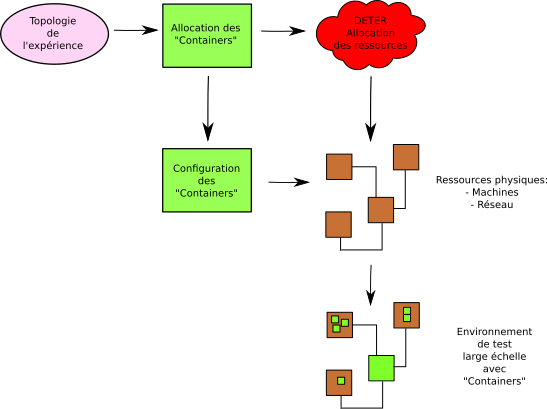
\includegraphics[scale=0.75]{Pictures/png/Deter_fonctionnement_container_v2}
  \caption{Diagramme du fonctionnement d'un \textit{Container}}
  \label{Conteneur}
\end{figure}

Ensuite, on trouve le simulateur DASH\footnote{Deter Agents Simulating Humans}
qui permet de prédire le comportement humain en se basant sur des modèles de
pensées, de réactions aux évènements et de comportements instinctifs ou
délibérés.

Dans la réalité, lors de cyber-attaques ou cyber-defenses, chaque
partie n'a qu'une vision partielle du monde. Par exemple, dans le cas
d'un système anti-malware, le système a une vision complète de son
réseau local, mais sa vision de la topologie globale du réseau est
partielle. Le système doit donc prendre en compte ce facteur pour
toutes ses actions. Pour intégrer cela à DeterLab, les chercheurs du
projet DETER ont créé le ``Multi-party Experiments''. Cet outil permet
de configurer pour chaque entité d'une expérience le flux
d'information qu'elle diffuse et à qui, ainsi que son degré de
visibilité sur le réseau.

Actuellement, il existe plusieurs plateformes de tests basées sur
Emulab avec des extensions pour pouvoir être utilisées dans des
domaines spécifiques comme le fait DETER. Il se peut qu'une expérience
exécutée sur une de ces plateformes aie besoin de plus de machines que
la plateforme ne peut en fournir, que ce soit en terme de nombre, de
puissance ou d'hétérogénéité des machines. Pour pallier ce problème le
projet DETER a créé la
``Federation''\citep{DETER_faber2007deter}. Elle permet de déployer
une expérience sur plusieurs plateforme de tests différentes. La
Fig.\ref{Federation} montre l'éxécution d'une expérience dont les 3
n\oe uds sont répartis sur différentes plateformes. La difficulté ici
est que les plateformes sont controllées par des propriétaires
différents ayant des règles de sécurité d'accès souvent très
différentes de celles du projet DETER.

\begin{figure}
  \centering 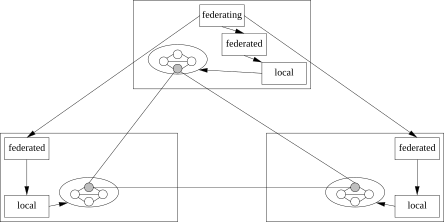
\includegraphics[scale=0.75]{Pictures/png/Deter_federation}
  \caption{Fédération d'une experience réparties sur 3 plateformes de tests différentes}
  \label{Federation}
\end{figure}

Pour que cette solution fonctionne les plateformes vont partager un
système de nommage permettant de ne pas montrer à l'application la
répartition de ses ressources sur le réseau, une authentification pour
contrôler l'accès d'une plateforme à une autre. Pour gérer cela on va
utiliser trois types de n\oe uds différents (Fig\ref{Federation}). Le
premier est le ``federating'', il est unique et se place sur la
plateforme qui demande à exécuter une expérience. Il cherche les
ressources disponibles sur les différentes plateforme puis divise
l'expérience en sous-expérience qu'il assigne à chaque plateforme. Il
gère l'exécution de l'expérience et récupère les données à la fin de
l'expérience et libère les ressources utilisées. Le second type de n
\oe ud est le ``federated'', on en place un sur chaque
plateforme. C'est lui qui fournit la liste des ressources disponibles
sur sa plateforme de tests et qui configure les sous-expériences qu'il
reçoit du federating. Il fait la traduction de nom entre le
federating, qui utilise le système de nommage partagé, et le reseau
local qui utilise son système de nommage spécifique.  Il gère
également la mise en place des connexions réseaux entre les entités
réparties sur les différentes plateformes. Le dernier n\oe uds appelé
``local'' est également présent sur chaque plateforme où l'expérience
va s'exécuter. Il gère les communications entre les différentes
plateforme et les sécurise pour éviter les fuites à l'extérieur du
réseau ou l'espionnage par d'autres applications s'exécutant sur la
même plateforme.

MAGI\footnote{Montage AGent Infrastructure} fournit un système de
gestion de flux entre les différentes entités d'une expérience,
permettant ainsi d'avoir un certain contrôle sur les machines. En
gérant le flux on peut automatiser et reproduire les expériences. En
effet, MAGI capture chaque séquence d'instructions concurrentes que
l'expérience va suivre pour gérer le flux, ainsi on peut rejouer la
capture plus tard avec les paramètres d'origine ou des nouveaux si un
fichier de paramètres à tester existe. MAGI permet également de
visualiser l'évolution d'une expérience en cours d'exécution pour
s'assurer que son comportement reste correct sans avoir à attendre le
résultat final. En capturant les configurations demandées par les
utilisateurs MAGI permet leur réutilisation par d'autres utilisateurs
pour éviter à DETER de reconstruire la même architecture plus tard.

Pour finir DETER a créé un outil appelé ``Risky Experiment Management
Capability'' qui permet de contrôler les expériences ayant besoin d'un
accès à l'extérieur (Internet, ou réseau de la plateforme externe à
celui d'exécution). Selon le risque des applications elles n'ont pas
toutes les mêmes restrictions. Si une application ne prend aucune
mesure de sécurité pendant son exécution alors l'environnement
d'exécution sera contrôlé voir isolé du reste du réseau. Dans le cas
contraire elle peut avoir la possibilité d'accéder à l'extérieur selon
sa criticité avec plus ou moins de droits, cela permet d'avoir des tests encore plus
réalistes. Pour cela l'outil va placer des portes vers l'extérieur
dans l'infrastructure de l'expérience. Ces portes ne seront pas
totalement libres, pour chacune on spécifie le chemin d'entrée et de
sortie de l'infrastructure pour un traffic spécifique et l'adresse de
la source ou de la destination.

\begin{figure}[H]
\centering
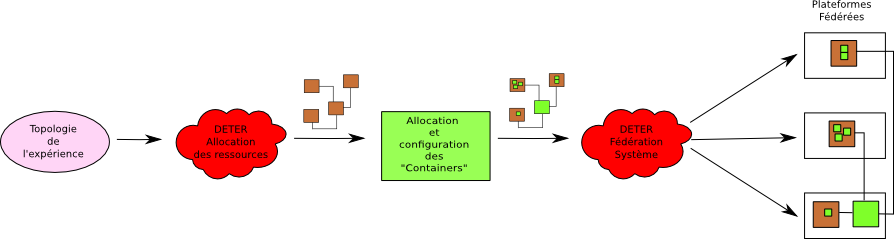
\includegraphics[scale=0.63]{Pictures/png/Deter_fonctionnement_general}
\caption{Création de l'environnement d'une expérience}
\label{Deter_fonc}
\end{figure}

De par les tests que la plateforme va effectuer il faut bien la
sécuriser. En effet, elle pourrait subir des attaques externes ou
internes. DETER propose un système de fichier crypté pour contrer
l'espionnage interne, un firewall pour éviter les fuites vers
l'extérieur, une IDS pour éviter les intrusions.

 Actuellement, DeterLab peut émuler des dizaines de milliers de n\oe
 uds, le projet dispose de 500 machines et 10 FPGA. Il est le seul
 émulateur dans le domaine de la cyber-sécurité et permet de faire des
 tests large échelle dont la complexité est représentative des
 réseaux. \textit{Dernièrement de nouvelles expériences sont apparues
   dans les domaines de la sécurité des réseaux avionique et la
   robustesse de l'anonymat sur le réseau. De plus, des exercices et
   des cours concernant les outils fournis par DeterLab et les
   méthodes expérimentales développées au sein du projet DETER sont
   mis à disposition des enseignants en cyber-sécurité et de leurs
   étudiants.}\textbf{à mettre ou pas?}
